\section{Arquitectura y diseño del sistem}

\subsection{Descripción General del código}

La transición del entorno científico de los Jupyter Notebook a un sistema de producción automatizado requiere una arquitectura de software ordenada. Para garantizar principios de Ingeniería de Software como la escalabilidad, la mantenibilidad y la separación de responsabilidades, el sistema fue diseñado bajo el paradigma de la Programación Orientada a Objetos (POO) y empleando patrones de diseño. Las funciones principales son:

\begin{itemize}
	\item Automatización: Ejecutar toda la tubería de datos o \emph{pipeline} (limpieza, partición, escalado, entrenamiento y evaluación) de maneta automatizada.
	\item Reproducibilidad: Garantizar que las transformaciones estadísticas se aprendan exclusivamente del conjunto de entrenamiento y se apliquen de forma consistente a datos nuevos. 
	\item Persistencia: Generar y guardar automáticamente los artefactos del modelo (.joblib y .pth) para su posterior uso.
\end{itemize}

\subsection{Estructura del directorio}

La estructura del código está organizando los archivos en capas lógicas:

\begin{verbatim}
|-- data/
|   |-- dataset_builder.py      # Capa de construcción e integración de datos crudos
|-- features/
|   |-- pipeline.py             # Capa de preprocesamiento
|-- models/
|   |-- base.py                 # Interfaz abstracta de modelado
|   |-- supervised.py           # Algoritmos predictivos (Red Neuronal, Regresión)
|   |-- unsupervised.py         # Algoritmos descriptivos (PAM Clustering)
|-- views/
|   |-- reports.py              # Capa de presentación (UI/Consola)
|-- pipeline_controller.py      # Controlador principal
|-- demo.py                     # Simulador basado en los modelos
\end{verbatim}

\subsection{Patrones de Diseño}

\textbf{1. Modelo-Vista-Controlador (MVC)} \\
La arquitectura general del código se divide en las principales componentes de un sistema:
\begin{itemize}
	\item \textbf{Modelo (\texttt{src/models}, \texttt{src/features}, \texttt{src/data}):} Capa lógica. Encapsula toda la matemática, algoritmos y la manipulación de datos.
	\item \textbf{Vista (\texttt{src/views/reports.py}):} Capa de salida que contiene las impresiones en pantalla para el usuario.
	\item \textbf{Controladores (\texttt{pipeline\_controller.py} y \texttt{demo.py}):} Capa de control. Dirigen el flujo de datos desde su ingesta hasta transformación en conocimiento útil mediante los modelos.
\end{itemize}
\textit{Justificación:} Esta arquitectura garantiza que futuras modificaciones en alguna capa no alteren la lógica de las demás, en particular la de capas complejas como el Controlador, brindando un alto desacoplamiento.
\newpage
\textbf{2. Strategy (Estrategia)} \\
Implementado en el directorio \texttt{models/}. \\
Se diseñó una interfaz abstracta base (\texttt{ModeloEstrategia}) que actúa como contrato, obligando a todas las clases algorítmicas concretas (\texttt{RedNeuronalEstrategia}, \texttt{PamClusteringEstrategia}) a implementar los métodos homólogos: \texttt{entrenar()}, \texttt{predecir()}, \texttt{guardar()} y \texttt{cargar()}. \\
\textit{Justificación:} Otorga al sistema la capacidad de polimorfismo. Permite al controlador intercambiar dinámicamente un algoritmo de Regresión Logística por una Red Neuronal Profunda sin modificar la lógica compleja subyacente, cumplimiendo el Principio de Abierto/Cerrado de SOLID, permitiendo extender las capacidades algorítmicas del sistema sin alterar el código existente.

\textbf{3. Builder (Constructor)} \\
Implementado en la clase \texttt{ConstructorDatasetHistorico}. \\
\textit{Justificación:} La desnormalización de la Base Histórica (ejecutando \textit{Joins} iterativos contra 13 dimensiones categóricas) y la posterior extracción de una muestra estratificada constituye un proceso de inicialización altamente complejo. El patrón \textit{Builder} separa la construcción matemática de este objeto de su representación final. Permite que el controlador principal consuma el \textit{dataset} limpio con un solo comando, abstrayendo su complejidad.

\textbf{4. Pipeline (Tubería)} \\
Implementado en la clase \texttt{RiesgoCreditoPipeline}. \\
\textit{Justificación:} Secuencia y estandariza las transformaciones matemáticas: imputación, escalado (\textit{RobustScaler}) y codificación (\textit{One-Hot Encoding}).Garantizar que cualquier dataset sea sometido exactamente a los mismos parámetros aprendidos durante la fase de entrenamiento, anulando cualquier discrepancia o sesgo.

\subsection{Diagrama de Clases UML}
El diseño se expone en el siguiente diagrama UML, el cual describe las clases con sus atributos y comportamiento, además de la relación que hay entre cada una:

\begin{figure}[H]
	\centering
	\vspace{10pt}
	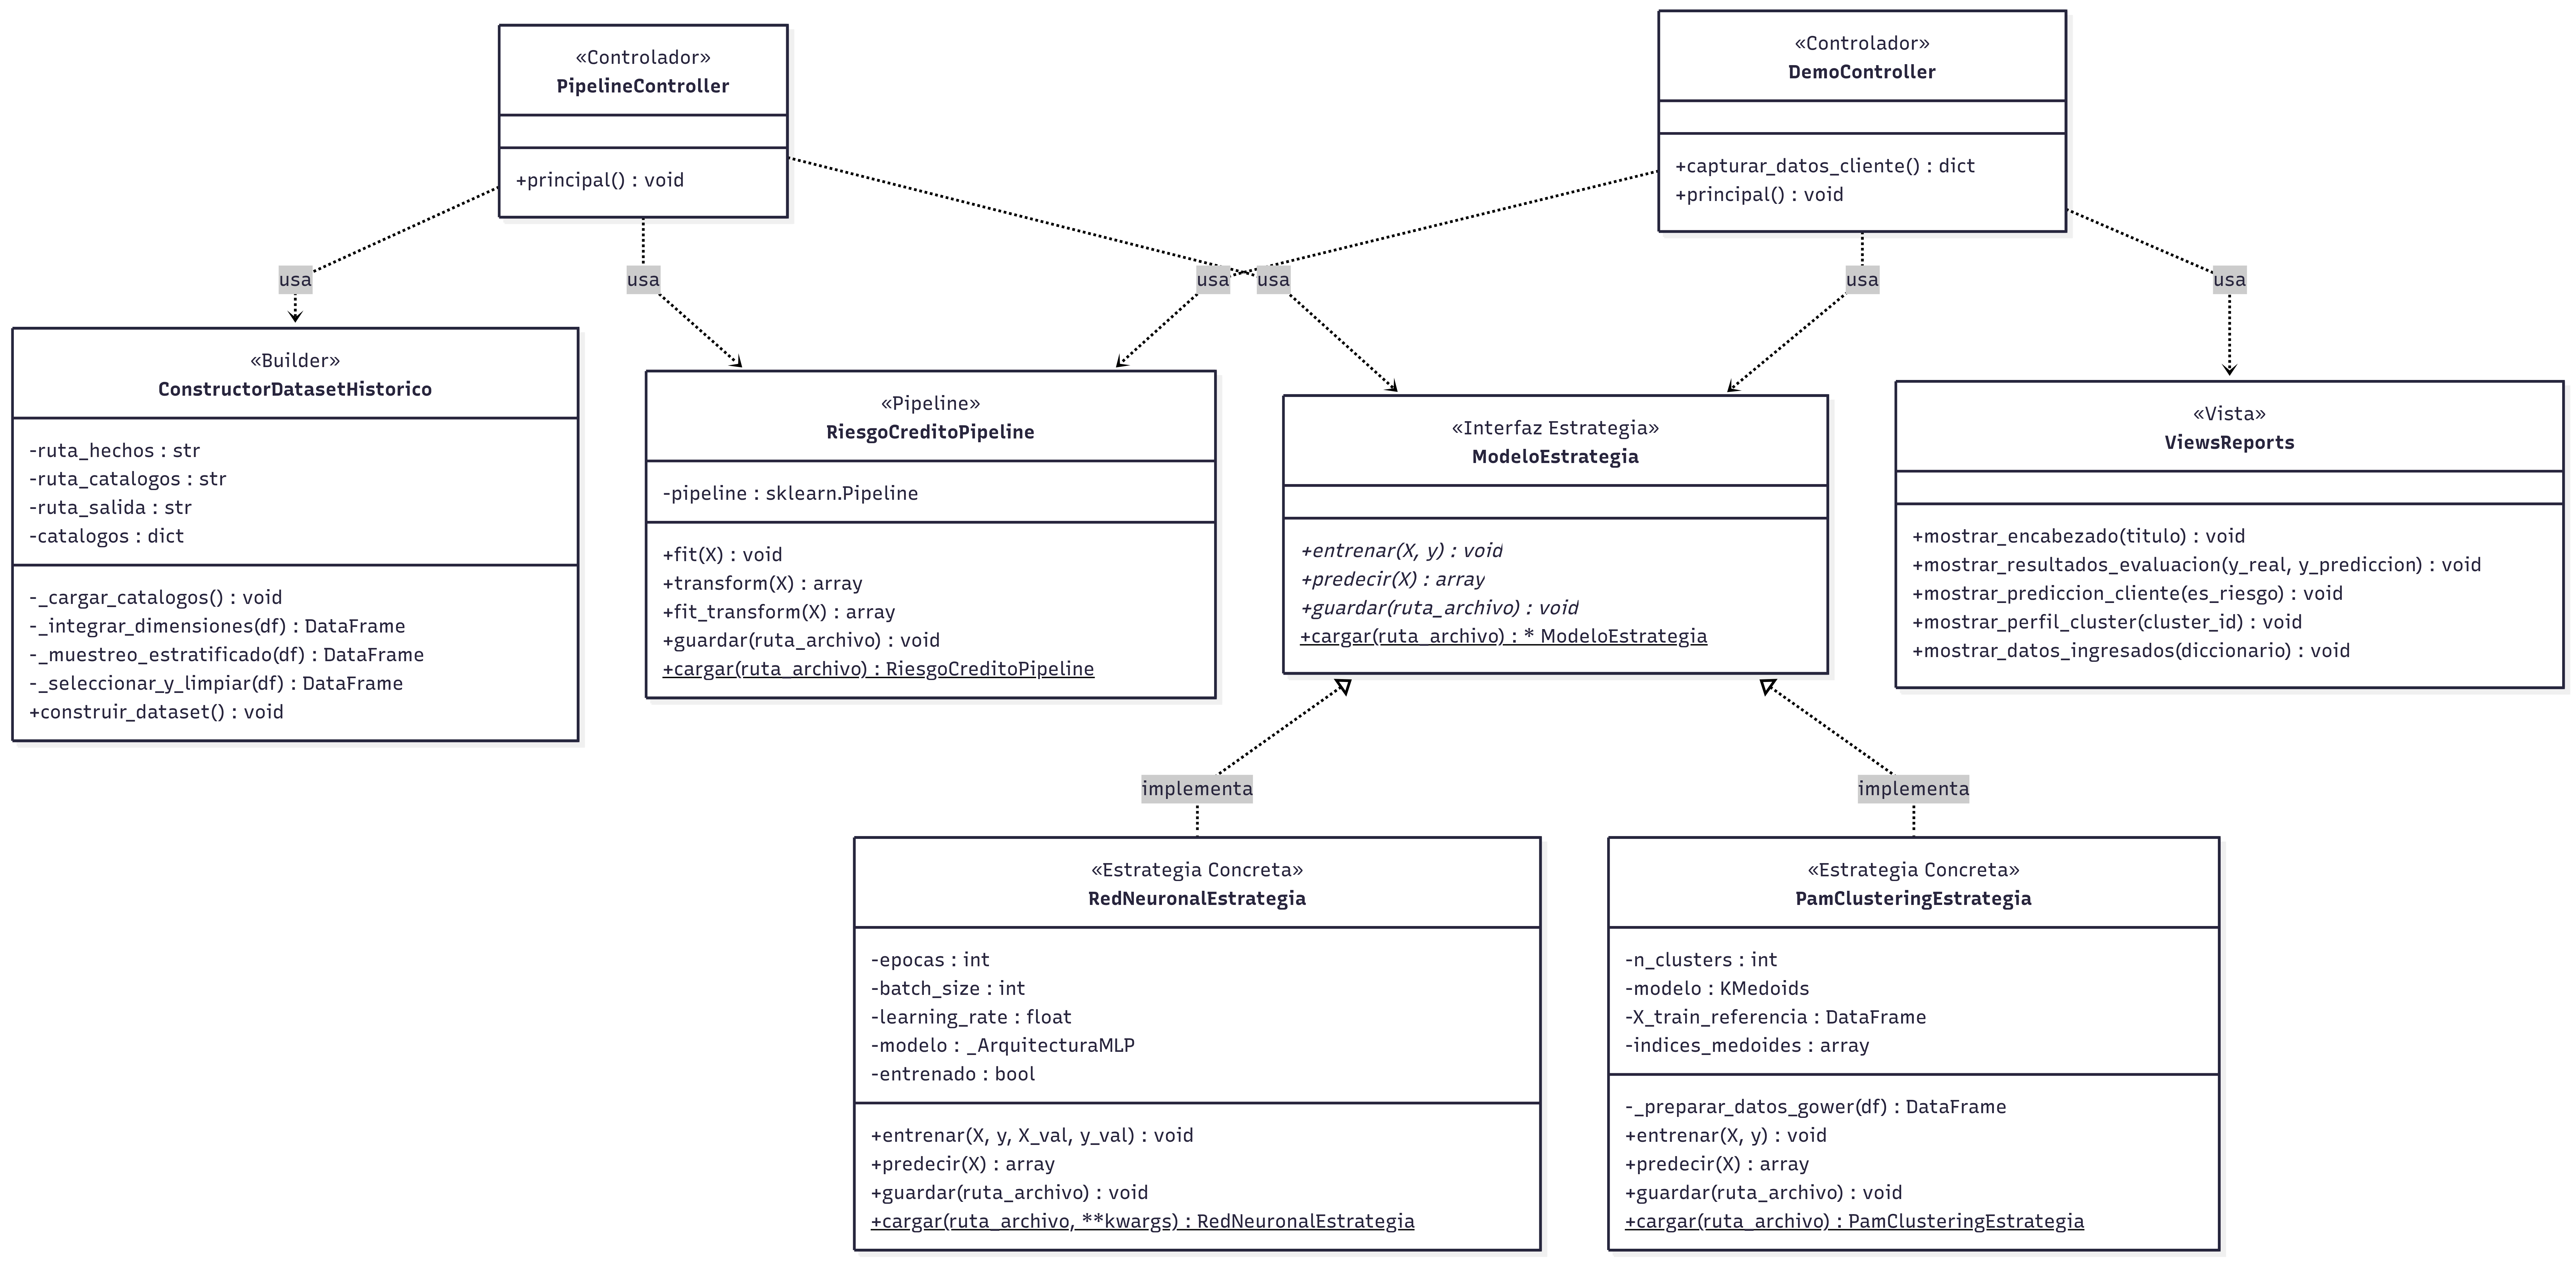
\includegraphics[scale=0.06]{imagenes/Capturas/diagram-UML.png}
	\caption{Diagrama UML del código estructurado en \texttt{src/}}
	\vspace{-20pt}
\end{figure}